\chapter{Implementation}

The implementation of the presented simulation is based on a previous simulation that can be found on the CoVprehension website \cite{covprehension_question_17_2020, adam:hal-03613433}. CoVprehension is a project independent of any organisation and initiated by researchers during the COVID-19 pandemic. The goal of this project is not to predict, but to explain in a simple way, with a scientific background, the evolution of the epidemic and its potential outcomes. In order to achieve this goal, different stages of the epidemic and ideas on how to battle it have been summarised into questions which, in turn, lead to explanations accompanied by sketches, diagrams and interactive simulations.

The previous simulation took as basis question 17 of CoVprehension \cite{covprehension_question_17_2020}: "Let{\textquoteright}s test people! Sure, but who, when and how?" Simply put, it shows how handling the epidemic through the use of screening tests is far from easy. Depending on the testing strategy, the constraint of limited available test kits and the delayed start of the campaign, different outcomes are obtained and may lead to decisions based on insufficient data.

Some changes were made to this previous simulation of question 17. Looking at the epidemiological model, the Incubation state was removed, and two new states were added: Hospitalised and Deceased. The Incubation state is not needed as it cancels itself out when updating trust levels and would bring, in this simulation, a useless delay before changing into a Symptomatic or an Asymptomatic state.
Within agents' attributes, everything related to testing and quarantine was removed, while a vaccination status and a trust level attribute were added. Keeping the testing and the quarantine parameters would have lengthened the duration of the simulation and over-complicated it. Instead, agents will directly know in which epidemiological state they and others are (except for asymptomatic agents, which are viewed and mistaken as susceptible agents). Finally, a number of methods were added, mostly in order to create a hospitalised area with visiting agents and interactions to update trust levels.

The source code, excluding the graphics user interface, is made of approximately 800 lines and is available on GitHub.\footnote{Source code: \url{https://github.com/CalvinMT/TrustVaccSim}} It was implemented and tested on NetLogo 6.2.2 using a 4 core CPU for which attaining 100 simulation ticks at normal simulation speed took around 7 seconds. Running the same code on NetLogo Web is possible\footnote{Simulator on NetLogo Web: \url{https://www.netlogoweb.org/launch\#https://raw.githubusercontent.com/CalvinMT/TrustVaccSim/main/src/trustvaccsim.nlogo}}, yet slower, reaching 100 simulation ticks with a normal simulation speed at around 23 seconds. A screenshot of the simulation on NetLogo Web can be viewed in figure \ref{fig:simulation_screenshot}.


\section{Simulation specifications}

\begin{figure}
    \centering
    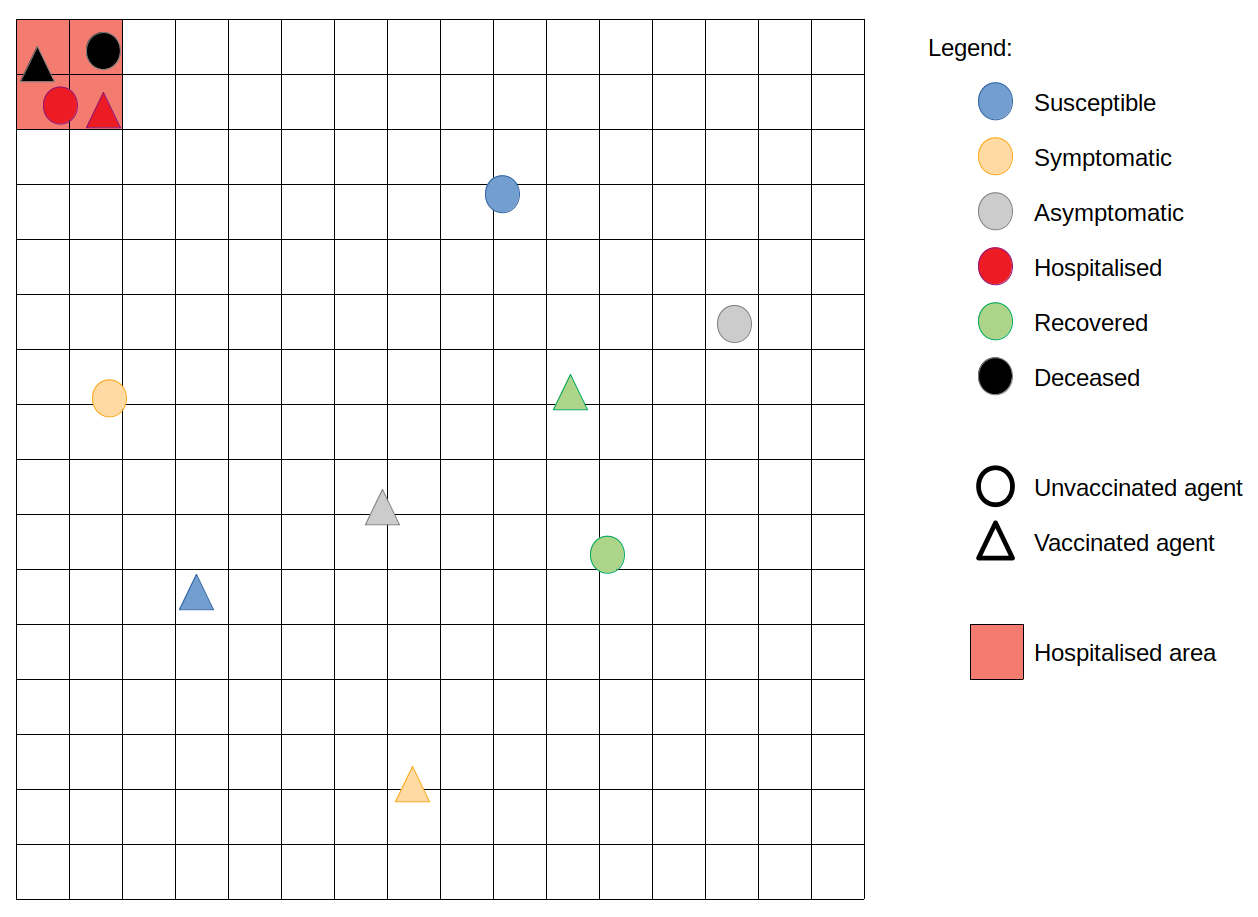
\includegraphics[width=0.9\linewidth]{pics/simulation_figure.png}
    \caption{Visual outline of the environment of the simulator.}
    \label{fig:simulation_environment}
\end{figure}

The environment of the simulation consists of a square of 256 patches (16x16) in which a population of 2000 agents is equally distributed between all patches other than those considered the hospitalised area. The hospitalised area is situated in the top-left corner of the environment and takes up a square of 4 patches (2x2). Simply put, a patch, in NetLogo, is a square with accessible properties that composes the environment on which agents can wander and perform their activities.

Each agent starts in the Susceptible state, with exception to one randomly chosen agent initialised with the Symptomatic state. Once the simulation starts, agents move around freely and randomly in the environment, avoiding the hospitalised area. Agents on the same patch are considered close enough for airborne transmission of the virus, as through the means of aerosols. Thus, if one of them is infectious, other agents on the same patch and in the Susceptible state have a risk of getting infected, putting them either in the Symptomatic or Asymptomatic state. If in the Hospitalised state, agents are moved into the hospitalised area, as if taken into a hospital. They will stay in that area without infecting anyone until they recover from the disease. Hospitalised agents are visited by ten other randomly chosen non-hospitalised agents for 5 simulation steps.

An agent's colour informs the user of the simulation on its epidemiological state, while its shape notifies on its vaccination status. Blue is Susceptible, yellow is Infected, grey is Asymptomatic, red is Hospitalised, green is Recovered and black is Deceased. Once an agent falls into the Deceased state, it stops moving and vanishes over time. As agents pop in and out of the hospitalised area, the choice was made to make agents that fall into the Deceased state gradually vanish instead of directly disappear so that the user can clearly identify when agents go from a Hospitalised state to a Deceased state. Additionally, they are not left visible in the simulation, or they would, in some scenarios, rapidly fill the hospitalised area. Concerning the vaccination status, an agent represented as a circle is unvaccinated and an agent drawn as a triangle is vaccinated.
A visual outline of the environment of the simulator is observable in figure \ref{fig:simulation_environment}.


\section{Entry parameters}
\label{entry_parameters}

The simulation enables users to modify a single of its entry parameters. This simplicity in the simulation allows the user to focus solely on the effect of this parameter alone over the entire model, thus making it easier for the user to observe what the simulator is intended to show them.

The modifiable entry parameter is the initial average trust of the population. This parameter is identified as a slider ranging from 0.1 to 0.9 with steps of 0.1. A population with an average trust of 0.1 is considered representative of a highly distrusting population, while a population considered highly trusting would have an average trust of 0.9. This average trust is initialised using a custom distribution algorithm as shown in figure \ref{fig:initial_average_trust}. This method was chosen for its simple implementation and in order not to limit the range of randomly chosen trust levels as a normal distribution would, but closer to what a skew normal distribution would give.

\begin{figure}[!htb]
    \centering
    \minipage{0.6\textwidth}
        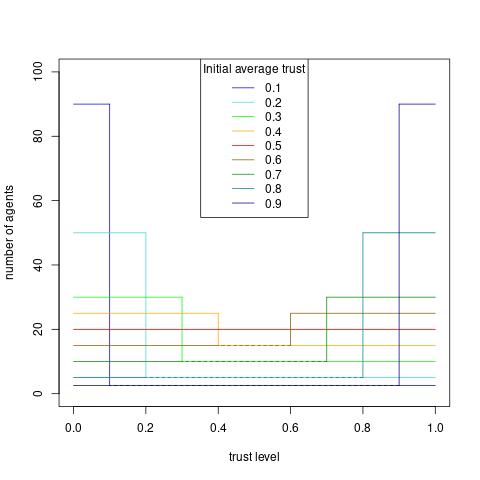
\includegraphics[width=\linewidth]{pics/initial_average_trust.png}
        \caption{Output of the algorithm used in the initialisation of the population's average trust.}
        \label{fig:initial_average_trust}
    \endminipage{}
\end{figure}

\pagebreak

The idea behind the trust level initialisation algorithm is simple and goes as follows. For all agents, if the current population's average trust --- a floating point initialised at 0 --- is below the user-set initial population's average trust, then the trust level of the current agent is randomly set between $X$ and 1. $X$ being the opposite number to the current population's average trust level, based on the user-set initial average trust level. Although, if $X$ is above 1, it is set to 0.9. And if $X$ is below 0, it is set to 0.1. Otherwise, if the current population's average trust is above the user-set initial population's average trust, this time the current agent's trust level is randomly set between 0 and $X$. Finally, if the current population's average trust is equal to the user-set initial population's average trust, the current agent's trust level is set between 0 and 1. See algorithm \ref{algo:initialisation_trust_level}.


\section{Outputs}
\label{implementation_outputs}

The user can visualise the environment in which agents wander around. This enables the user to observe agents changing from one epidemiological state to another by their colour and change vaccination status by their shape. Through this visualisation, the user can identify if the hospitalised area is more or less crowded.

A number of graphical outputs are also displayed to the user in order to follow the evolution of different variables:
\begin{itemize}
    \item Epidemic dynamic --- Percentage of agents over time for all epidemiological states, as well as the percentage of vaccinated agents over time and the average trust level of the population.
    \item Level of trust per interpretation status --- Average trust level of the correctly interpreting population and incorrectly interpreting population over time.
    \item Deaths per vaccination and interpretation statuses --- Number of deceased, unvaccinated and misinterpreting agents over time with the number of deceased, unvaccinated and correctly interpreting agents over time next to the number of deceased, vaccinated and misinterpreting agents over time followed by the number of deceased, vaccinated and correctly interpreting agents over time.
\end{itemize}

These visualisations were chosen to enable the user to make multiple key observations aiming at the goal of the present work. The user may observe the evolution of the epidemic, of the vaccination campaign, and of the population's average trust with the help of the epidemic dynamic. The observation of the average trust level between two subgroups of the population having different interpretation of information may assist the user in understanding the influence of misinterpretation of information on the population's average trust level, as well as the differences in starting an epidemic with a high or a low population's average trust level. Finally, observing the sorted death rate may help the user appreciate the resulting effect of having incorrectly interpreted information, having been vaccinated or not.